%--------------------------------------------------------------------------------------------
% Plotting model output
%--------------------------------------------------------------------------------------------

\chapter{Visualization}
\label{chap:nhyd_atm_visualization}

This chapter discusses visualization tools that are specific to this core.  For instructions on visualization tools that may be used by all cores, such as Paraview, see Chapter \ref{chap:mpas_visualization}.

Since the MPAS input and output files are in netCDF format, a wide variety of software
tools may be used to manipulate and visualize fields in these files. As a starting point, several NCL \footnote{NCAR Command Language; \url{http://ncl.ucar.edu}}
scripts are provided in the {\tt graphics/ncl} sub-directory
of the main MPAS directory for making the basic types of plots illustrated in Figure \ref{fig:ncl_plots}. Each of
these scripts reads the name of the file from which fields should be plotted from the environment variable {\tt FNAME},
and all but the mesh-plotting script read the time frame to be plotted from the environment variable {\tt T}. To plot
a field from the first frame (indexed from 0) of the file {\tt output.2010-10-23\_00:00:00.nc}, for example, one would set the 
following environment variables 

\vspace{12pt}
{\tt > setenv FNAME output.2010-10-23\_00:00:00.nc}

{\tt > setenv T 0}
\vspace{12pt}

\noindent before running one of the scripts. In general, the specific field to be plotted from the netCDF file must be set 
within a script before running that script. 

\begin{figure}[htb]
\begin{center}
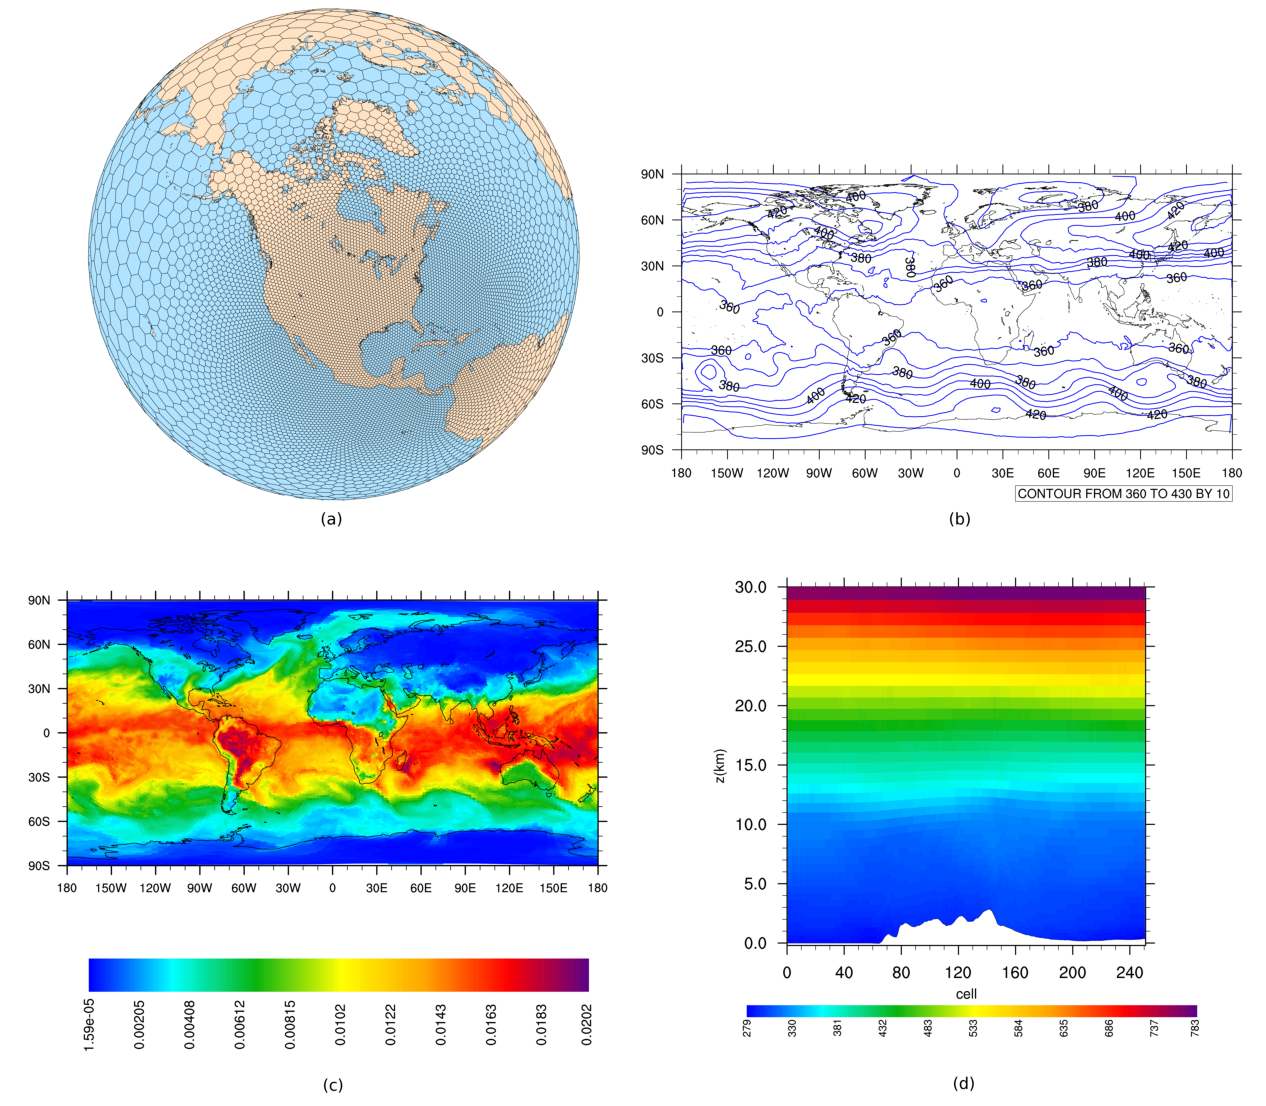
\includegraphics[width=6.5in]{nhyd_atm/figures/ncl_plots.pdf}
\caption{Various plot types that can be produced from MPAS input or output files using example scripts provided with the MPAS code.
(a) A plot of an MPAS SCVT mesh against a filled map background. (b) A simple horizontal contour plot. (c) A cell-filled horizontal plot, with
individual cells of the mesh drawn as polygons colored according to the field value. (d) A vertical cross-section in height, with areas below the
terrain left unshaded.}
\label{fig:ncl_plots}
\end{center}
\end{figure}


\section{Meshes}

A plot showing just an MPAS SCVT mesh can be produced using the {\tt atm\_mesh.ncl} script, as in Figure \ref{fig:ncl_plots}(a). This script
reads a subset of the mesh description fields in Appendix \ref{sec:var_sec_mesh} and uses this information to draw the SCVT mesh over a 
color-filled map background. Parameters in the script can be used to control the type of map projection (e.g., orthographic, cylindrical equidistant, etc.), 
the colors used to fill land and water points, and the widths of lines used for the Voronoi cells.


\section{Horizontal contour plots}

Contour plots of horizontal fields can be produced with the {\tt atm\_contours.ncl} script, as in Figure \ref{fig:ncl_plots}(b). The particular
field to be plotted is set in the script and can in principle be drawn on any horizontal surface (e.g., a constant pressure
surface, a constant height surface, sea-level, etc.) if suitable vertical interpolation code is added to the script. Not shown in the figure are horizontal
wind vectors, which can also be added to the plot using example code provided in the script.


\section{Horizontal cell-filled plots}

For visualizing horizontal fields on their native SCVT grid, the {\tt atm\_cells.ncl} script may be used to produce horizontal cell-filled plots, 
as in Figure \ref{fig:ncl_plots}(c). This script draws each MPAS grid cell as a polygon colored according to the value of the field in that
cell; the color scale is automatically chosen based on the range of the field and the default NCL color table, though other color tables can
be selected instead.


\section{Vertical cross-sections}

Vertical cross-sections of fields can be created using the {\tt atm\_xsec.ncl} script, as in Figure \ref{fig:ncl_plots}(d). Before running this script,
a starting point and an ending point for the cross section must be given as latitude-longitude pairs near the top of the script, and the number of points along
the cross section should be specified. The script evenly distributes the specified number of points along the shortest great-circle arc from the 
starting point to the ending point, and for each point, the script uses values from the grid cell containing that point (i.e., a nearest-neighbor interpolation
to the horizontal cross-section points is performed); no vertical interpolation is performed, and the thicknesses and vertical heights of cells are
all drawn according to the MPAS vertical grid.



